\documentclass[11pt, usepdftitle=false,...]{beamer}
\usetheme{default}

\usepackage[utf8]{inputenc}
\usepackage[german]{babel}
\usepackage{amsmath}
\usepackage{amsfonts}
\usepackage{amssymb}
\usepackage{graphicx}
\usepackage{pgf} 
\hypersetup{pdftitle=Implementierungsbericht}


\author{Denis Gensh, Marcel Herm, David Krah,\\
	Eduard Kukuy, Daniel Milbaier, Richard Rudolph}
\title{
	\textbf{Implementierungsbericht}
}
\subtitle{Workflow System für eine virtuelle Forschungsumgebung für
	Geodaten
	\vspace{-0.7cm}
	}
\logo{\pgfputat{\pgfxy(-1.7,8.0)}{\pgfbox[center,base]{
\includegraphics[scale=0.125]{logo.png}}}}
\institute{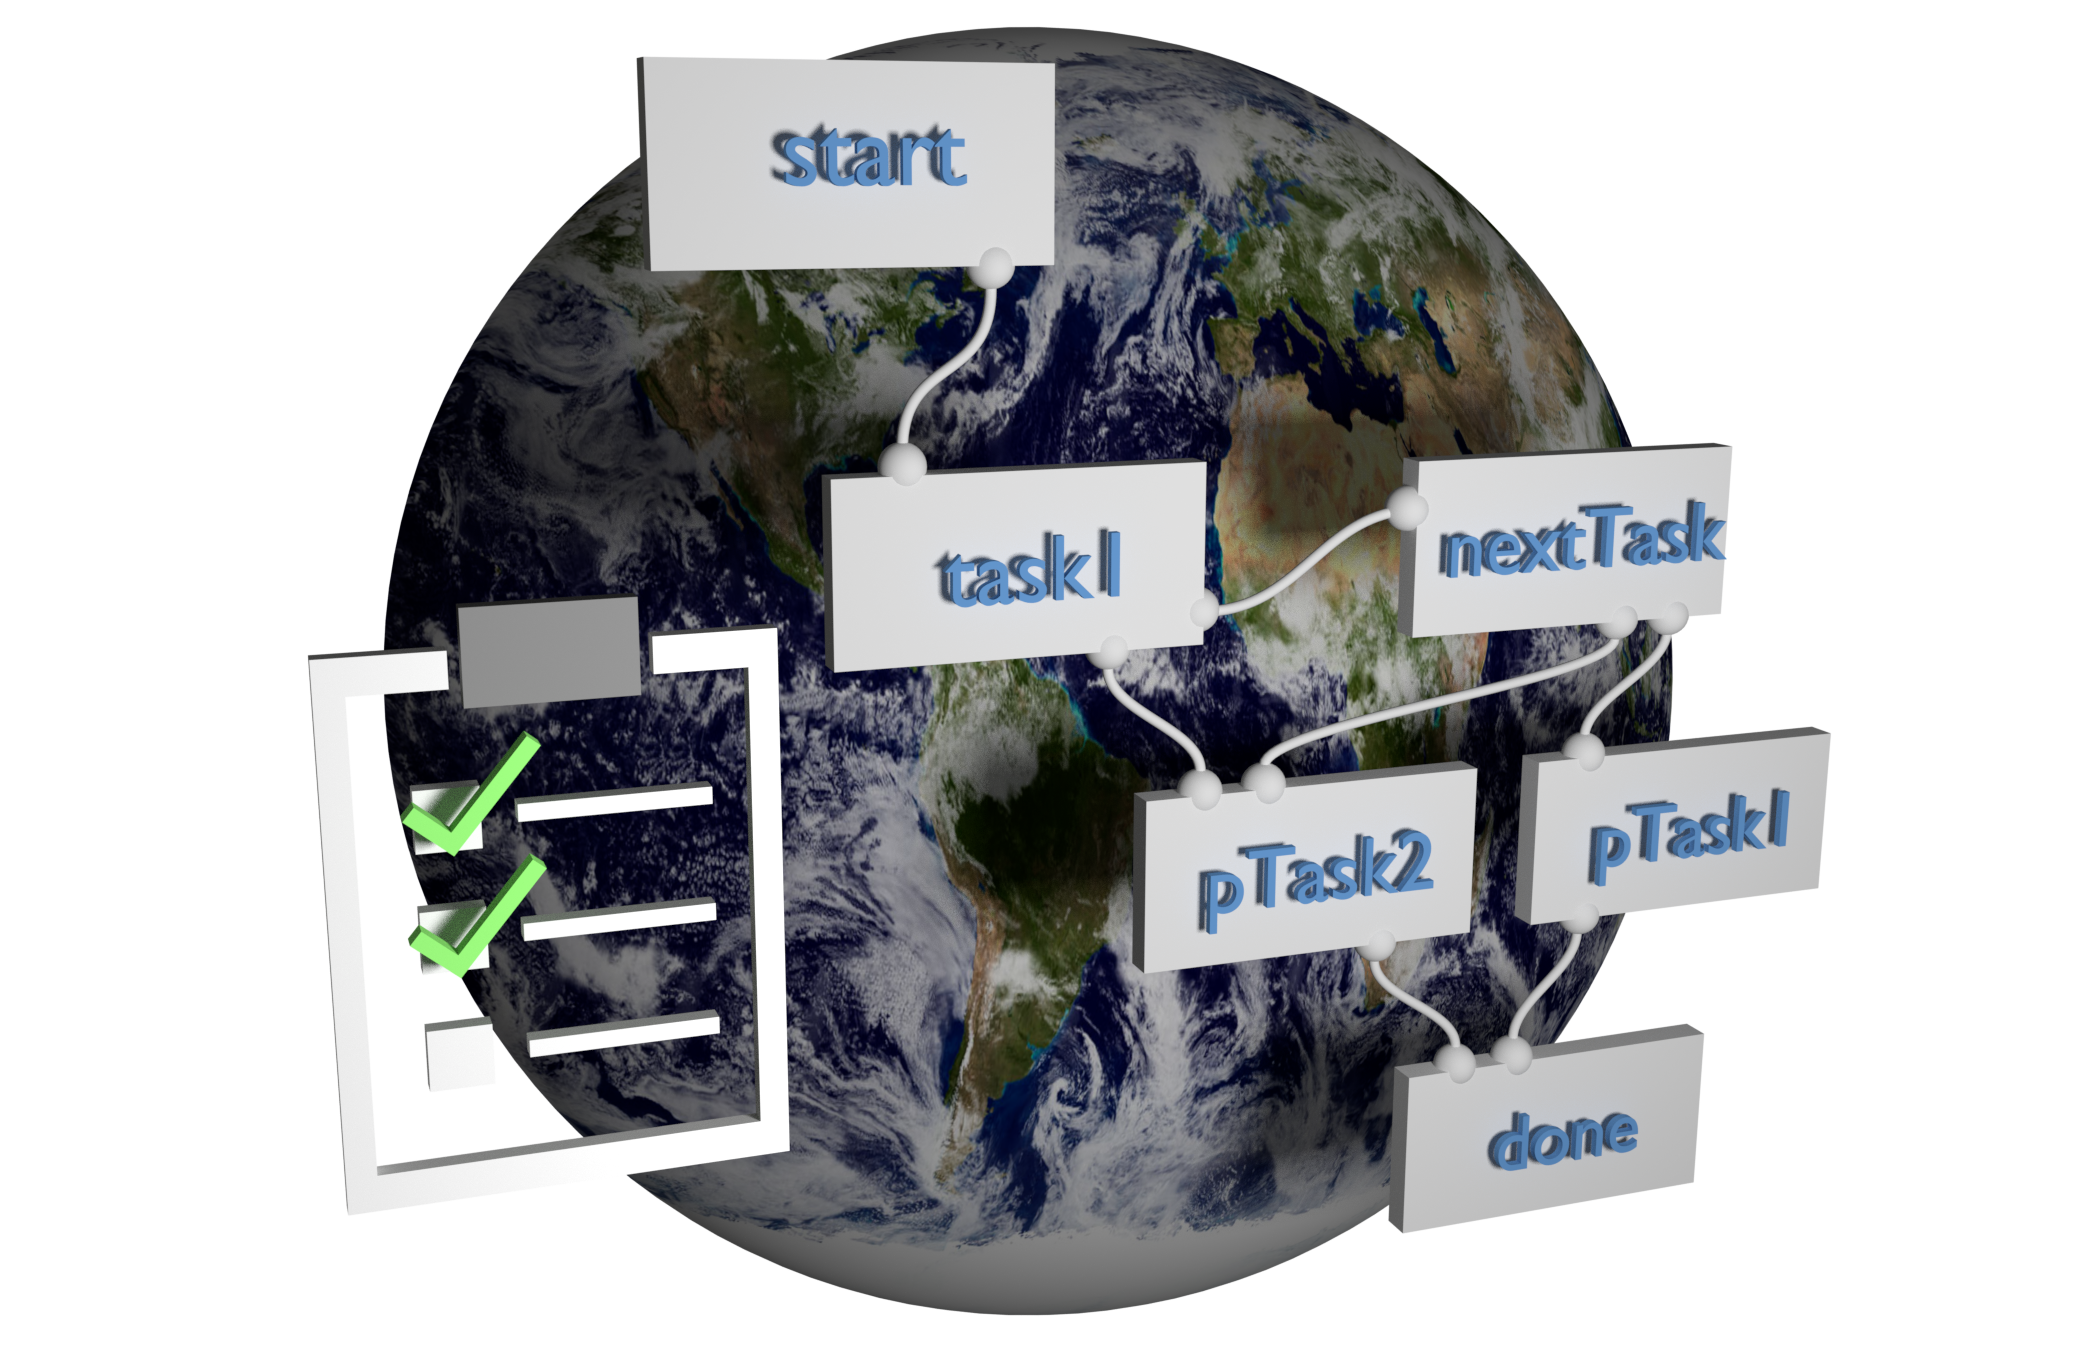
\includegraphics[height=3.5cm]{workflow2-tp3.png}}
\date{\today}
\subject{x}
%\setbeamercovered{transparent}
%\setbeamertemplate{navigation symbols}{}
\addtobeamertemplate{navigation symbols}{}{%
	\usebeamerfont{footline}%
	\usebeamercolor[fg]{footline}%
	\hspace{1em}%
	\insertframenumber/\inserttotalframenumber
}

\makeatletter
\setbeamertemplate{frametitle}{
	\ifbeamercolorempty[bg]{frametitle}{}{\nointerlineskip}%
	\@tempdima=\textwidth%
	\advance\@tempdima by\beamer@leftmargin%
	\advance\@tempdima by\beamer@rightmargin%
%	\hspace*{0} %%%%%%%%%%%%% For example insert shift to right
	\begin{beamercolorbox}[sep=0.5cm,left,wd=\the\@tempdima]{frametitle}
		\usebeamerfont{frametitle}%
		\vbox{}\vskip-1ex%
		\if@tempswa\else\csname beamer@ftecenter\endcsname\fi%
		\strut\insertframetitle\strut\par%
		{%
			\ifx\insertframesubtitle\@empty%
			\else%
			{\usebeamerfont{framesubtitle}\usebeamercolor[fg]{framesubtitle}\insertframesubtitle\strut\par}%
			\fi
		}%
		\vskip-3ex%
		\if@tempswa\else\vskip-.3cm\fi% set inside beamercolorbox... evil here...
	\end{beamercolorbox}%
}
\makeatother

\begin{document}
	{
		% no page #, no logo on title page
		\setbeamertemplate{footline}{}
		\setbeamertemplate{logo}{}
		\setbeamertemplate{navigation symbols}{}
		\begin{frame}
			\titlepage
		\end{frame}
	}
	
	%\maketitle
	
	
	\begin{frame}
		\frametitle{Inhaltsverzeichnis}
		\tableofcontents
	\end{frame}
	
	\section{Features}
	\frame{\sectionpage}
	
		\subsection{Implementierte Kriterien}
%		\frame{\subsectionpage}
		
%			\begin{frame}
%				\frametitle{Musskriterien}
%				\begin{itemize}
%					\item Verwalten von Web Processing Service Workflows
%					\begin{itemize}
%						\item Erstellen, Bearbeiten, Speichern, Laden, Anzeigen von Workflows
%						\item Auflistung von Workflows mit Ausführungsstatus
%						\item Wiederherstellung der letzten Sitzung
%						\item Fehlermanagement
%						\begin{itemize}
%							\item Editorprüfung auf Kompatibilität von Tasks innerhalb eines Workflows
%						\end{itemize}
%						\item Workflows und Tasks auf Syntax und Kompatibilität prüfen
%						\item Erstellen und Bearbeiten in grafischem Drag and Drop Editor
%						\item Dynamisches einbinden von neuen Web Processing Service Tasks in den Editor
%					\end{itemize}
%				\end{itemize}
%			\end{frame}
			
%			\begin{frame}
%				\frametitle{Musskriterien}	
%				\begin{itemize}
%					\item Der Login-Status des Nutzers wird erfasst
%					\item Nutzerfreundlichkeit
%					\begin{itemize}
%						\item Einfache, intuitive Benutzung des Editors
%					\end{itemize}
%					\item Open-Source
%					\item Hilfesektion für Benutzerfragen
%				\end{itemize}
%			\end{frame}
			
%			\begin{frame}
%				\frametitle{Wunschkriterien}
%				\begin{itemize}
%					\item Logging aller Aktivitäten
%					\item Detailansicht einzelner Workflows
%					\item Erweiterte Konfigurationseinstellungen
%					\item Installations-/Einrichtungsassistent
%				\end{itemize}
%			\end{frame}
			
%			\begin{frame}
%				\frametitle{Zusätzlich}
%				\begin{itemize}
%					\item Auflistung der Resultate
%					\item Ausgabe von Fehlern
%					\item Sortieren der Prozesse nach Server
%				\end{itemize}						
%			\end{frame}				
			
	
		\subsection{Gestrichene Kriterien}
%		\frame{\subsectionpage}
%		
%			\begin{frame}
%				\frametitle{Was gestrichen wurde}	
%			\end{frame}
			
	\section{Änderungen am Entwurf}	
	\frame{\sectionpage}
	
	\section{Zeitplanung}
	\frame{\sectionpage}
	
	\section{Zahlen und Statistiken}
	\frame{\sectionpage}
	
		\subsection{Zahlen}
		\frame{\subsectionpage}
			\begin{frame}
				\frametitle{Ein paar Zahlen}
				\begin{itemize}
					\item Lines of Code: ca 15000
					\item Commits: ca 370 Commits
					\item Dateien:					
				\end{itemize}	
			\end{frame}
			
		\subsection{Statistiken}
		\frame{\subsectionpage}
		
			\begin{frame}
				\frametitle{GitHub Insights Pulse}
				\begin{figure}[ht] 
					\centering
					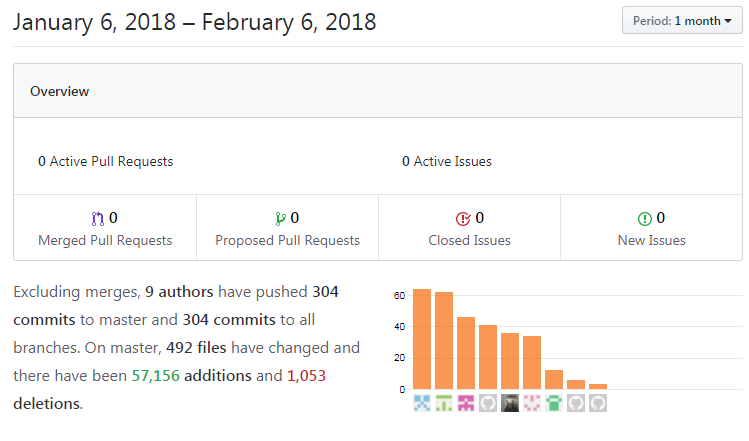
\includegraphics[scale=0.50, trim= 1cm 0 0 0]{pulse.png}
					\label{fig1}
				\end{figure}
			\end{frame}	
		
			\begin{frame}
				\frametitle{GitHub Insights Contributors}
				\begin{figure}[ht] 
					\centering
					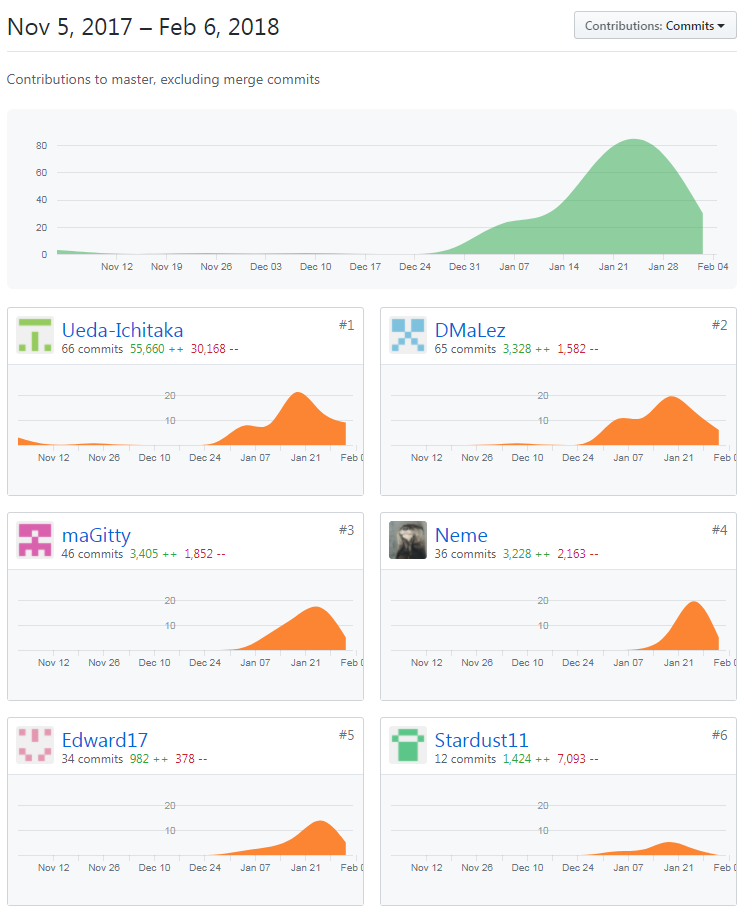
\includegraphics[scale=0.30, trim= 1cm 0 0 0]{contributors.png}
					\label{fig2}
				\end{figure}
			\end{frame}	
			
%			\begin{frame}
%				\frametitle{git fame}
%				\begin{figure}[ht] 
%					\centering
%					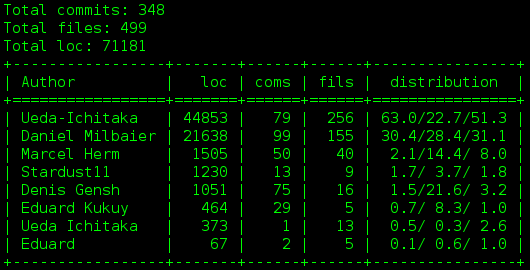
\includegraphics[scale=0.85, trim= .5cm 0 0 0]{git-fame.png}
%					\caption{git fame}
%					\label{fig1}
%				\end{figure} 
%			\end{frame}
%			
%			\begin{frame}
%				\frametitle{git lines}
%				\begin{figure}[ht] 
%					\centering
%					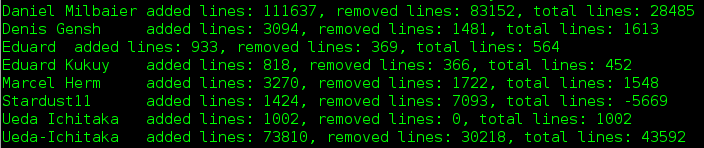
\includegraphics[scale=0.650, trim= 1cm 0 0 0]{git-lines.png}
%					\caption{git lines}
%					\label{fig2}
%				\end{figure} 
%			\end{frame}
	
			\begin{frame}
				\frametitle{List of authors}
				\begin{figure}[ht] 
					\centering
					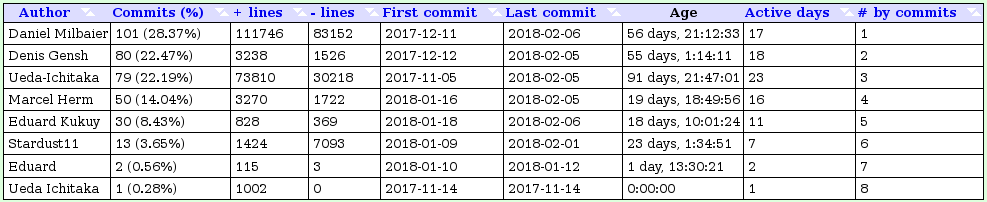
\includegraphics[scale=0.45, trim= 1cm 0 0 0]{authors.png}
					\label{fig3}
				\end{figure}
			\end{frame}
			
			\begin{frame}
				\frametitle{Lines of Code per Author}
				\begin{figure}[ht] 
					\centering
					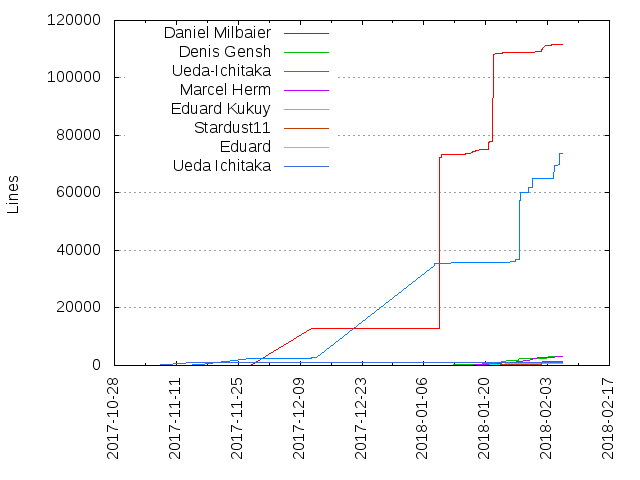
\includegraphics[scale=0.50, trim= 1cm 0 0 0]{lines_of_code_by_author.png}
					\label{fig4}
				\end{figure}
			\end{frame}
			
			\begin{frame}
				\frametitle{Commits per Author}
				\begin{figure}[ht] 
					\centering
					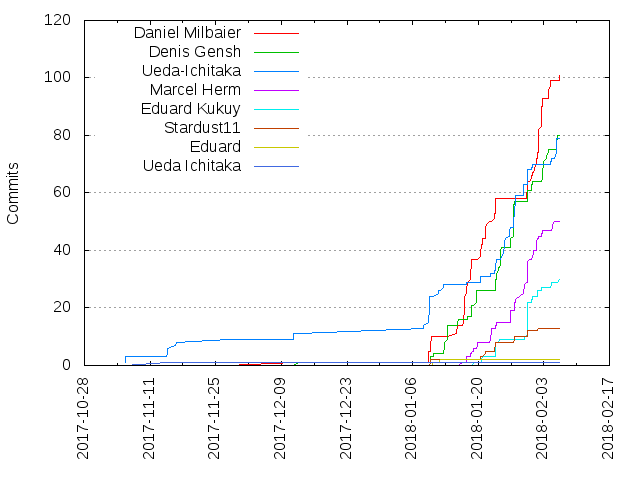
\includegraphics[scale=0.50, trim= 1cm 0 0 0]{commits_by_author.png}
					\label{fig5}
				\end{figure}
			\end{frame}
	
\end{document}